\documentclass[12pt]{book}
\usepackage{amsfonts,amsmath,amssymb,amscd,amsxtra,amsthm,verbatim,calc}
\usepackage{tikz}
\usetikzlibrary{cd}
\usetikzlibrary{patterns}
\usetikzlibrary{backgrounds}
\usepackage{amsmath}
\usepackage{amssymb}

\begin{document}

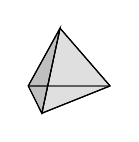
\begin{tikzpicture}[scale=0.6][line join = round, line cap = round]
	
	\coordinate (4) at (0,{sqrt(2)},0);
	\coordinate (3) at ({-.5*sqrt(3)},0,-.5);
	\coordinate (2) at (0,0,1);
	\coordinate (1) at ({.5*sqrt(3)},0,-.5);
	
	\begin{scope}
		\draw (1)--(3);
		\draw[fill=lightgray,fill opacity=.5] (2)--(1)--(4)--cycle;
		\draw[fill=gray,fill opacity=.5] (3)--(2)--(4)--cycle;
		\draw (2)--(1);
		\draw (2)--(3);
		\draw (3)--(4);
		\draw (2)--(4);
		\draw (1)--(4);
	\end{scope}
\end{tikzpicture}

\end{document}